\begin{frame}
	\frametitle{第六讲、级数收敛性的判定}
	\linespread{1.5}
	\begin{enumerate}
	  \item {\bf 内容与要求}{\color{blue}( \S2.4-2.5 )}
	  \begin{itemize}
%  	    \item 理解无穷级数的概念
%  	    \item 熟练掌握级数的基本性质
	    \item 熟练掌握同号级数收敛的判定方法
	    \item 掌握变号级数收敛的有关性质
	    \item 了解一些特殊的判别法
% 	  \vspace{1em}
	  \end{itemize}
	  \item {\bf 课后练习:}
	  \begin{itemize}
	    \item 书面作业:\\
	    \quad\quad{\b 习题2.4:1(2-4),3(3-8),5(2,4),6(1-3),8,9}\\
	    \quad\quad{\b 习题2.5:2(1,3,6,7,8),3,7,8}
	    \item 思考题:{\b 习题2.4:10-15,17;习题2.5:4,6,10,13}
	  \end{itemize}
	\end{enumerate}
\end{frame}

\section{同号级数的收敛性}

\begin{frame}{同号级数收敛性的判定}
	\linespread{1.6}
	\begin{enumerate}\pause
	  \item {\bf 收敛的充要条件}\pause
	  \item {\bf 比较判别法}\pause
	  \item {\bf 比值判别法}\pause
	  \item {\bf 根值判别法}\pause
	  \item {\bf Raabe判别法*}
	\end{enumerate}
\end{frame}

\begin{frame}{1、同号级数收敛的充要条件}
	\linespread{1.2}\pause
	\begin{block}{{\bf 定理2.4.1}\hfill P79}
		正项级数$\sumn a_n$收敛,当且仅当其部分和数列有界
	\end{block}\pause
	\bigskip
% 	\vspace{1em}
	\begin{exampleblock}{{\bf 例}\hfill P80-例1}
		证明$\sumn\df 1{n!}$收敛。
	\end{exampleblock}
% 	\pause
% 	\begin{alertblock}{{\bf $p$级数的敛散性}\hfill P81-例2}
% 		$\sumn\df 1{n^p}$当$p>1$时收敛;$0<p\leq 1$时发散。
% 	\end{alertblock}
\end{frame}

\begin{frame}{2、比较判别法}
	\linespread{1.2}\pause
	\begin{block}{{\bf 定理2.4.2}\hfill P81}
		设对充分大的$n$,总有$0\leq a_n\leq b_n$,则:\pause
		\begin{enumerate}
		  \item $\sumn b_n$收敛$\Rightarrow\sumn a_n$收敛\pause
		  \item $\sumn a_n$发散$\Rightarrow\sumn b_n$发散\pause
		\end{enumerate}
	\end{block}
	\begin{exampleblock}{{\bf 例}\hfill P82-例3}
		$0<p<1$时,$\sumn\df 1{n^p}$发散
	\end{exampleblock}
\end{frame}

\begin{frame}{$p$级数}
	\linespread{1.2}
	\begin{alertblock}{{\bf $p$级数的敛散性}\hfill P81-例2}
		$\sumn\df 1{n^p}$当$p>1$时收敛;$0<p\leq 1$时发散。
	\end{alertblock}\pause 
	\begin{exampleblock}{{\bf 例:}讨论下列级数的敛散性}\pause 
		\begin{columns}
			\column{.4\textwidth}
				\begin{enumerate}
				  \item $\sumn\df{1}{3^{\ln n}}$\pause 
				  \item $\sum\limits_{n=2}^{\infty}\df 1{(\ln n)^{\ln n}}$\pause 
				\end{enumerate}	
			\column{.6\textwidth}
				\begin{enumerate}
				  \addtocounter{enumi}{2}
% 				  \item $\sumn\df{1}{3^{\ln n}}$
				  \item $\sum\limits_{n=3}^{\infty}\df 1{(\ln n)^{\ln\ln n}}$\\[10pt]
				  \pause \hspace{-1em}\alert{[提示:$a^{\ln b}=b^{\ln a},\;(a,b>0)$]}
				\end{enumerate}
		\end{columns}
		
	\end{exampleblock}
\end{frame}

\begin{frame}
	\linespread{1.2}
	\begin{alertblock}{{\bf 例}\hfill P82-例4}
		设$a_n\leq c_n\leq b_n\;(n\in\mathbb{N})$,$\sumn a_n,\sumn b_n$均收敛,则$\sumn
		c_n$收敛。
	\end{alertblock}\pause
	\begin{itemize}
	  \item 级数收敛的“夹逼定理”\pause
% 	  \item {\ba{比较判别法仅对正项级数有效}}\pause
	\end{itemize}
	\begin{exampleblock}{{\bf 例}\hfill P93-定理2.5.2}
		若级数$\sumn|a_n|$收敛,则$\sumn a_n$也收敛。
	\end{exampleblock}
\end{frame}

\begin{frame}
	\linespread{1.2}\pause 
	\begin{block}{{\bf 定理2.4.3}(比较判别法的极限形式)\hfill P83}
		已知$a_n,b_n$均非负$(n\in\mathbb{N})$,且$\limn\df{a_n}{b_n}=l$,则\pause 
		\begin{enumerate}
		  \item 若$0<l<+\infty$,$\sumn a_n,\sumn b_n$同敛散\pause 
		  \item 若$l=0$,$\sumn b_n$收敛$\Rightarrow\sumn a_n$收敛\pause 
		  \item 若$l=+\infty$,$\sumn a_n$收敛$\Rightarrow\sumn b_n$收敛
		\end{enumerate}
	\end{block}
	\pause
	\begin{itemize}
	  \item \ba{比较判别法仅对同号级数有效}
	\end{itemize}
% 	\ba{注:}对非同号的级数该结论不成立
% 	\pause 例如:\\
% 	\centerline{$\sumn\df{(-1)^n}{\sqrt n}$\quad 和\quad 
% 	$\sumn\left[\df{(-1)^n}{\sqrt n}+\df 1n\right]$}
\end{frame}

\begin{frame}
	\linespread{1.6}
	\begin{exampleblock}{{\bf 例:}判断以下级数的收敛性\hfill P83-例5,6}\pause 
		\begin{enumerate}
		  \item $\sumn\df 1{2^n}\df{n^2+1}{2n^2-1}$\pause 
		  \item $\sumn\df{n+1}{n^k+2}\quad (k=1,2,\ldots)$\pause 
		  \item $\sumn\df{1}{n\sqrt[n]{n}}$\pause 
		  \item $\sumn\df{1}{1+x^n}\quad(x>0)$
		\end{enumerate}
	\end{exampleblock}
\end{frame}

\begin{frame}
	\linespread{1.2}
	\begin{block}{{\bf 推论1:}($p$-判别法)\hfill}\pause 
		设$a_n\geq 0\;(n=1,2,\ldots)$,则\pause 
		\begin{enumerate}
		  \item 若存在$p>1$,使得$\limn n^pa_n$存在,则$\sumn a_n$收敛\pause 
		  \item 若$0<p\leq 1$,使得$\limn n^pa_n>0$,则$\sumn a_n$发散
		\end{enumerate}
	\end{block}\pause 
	\begin{exampleblock}{{\bf 例:}判断以下级数的收敛性}
		\begin{enumerate}
		  \item $\sumn\df{\arctan n}{n^{3/2}}$\pause 
		  \item $\sumn\df{\ln n}{n^{5/4}}$
		\end{enumerate}
	\end{exampleblock}
\end{frame}

\begin{frame}
	\linespread{1.2}\pause
	\begin{block}{{\bf 推论2}}
		$\sumn a_n$、$\sumn b_n$均为正项级数,若对充分大的$n$,总有
		$$\df{a_{n+1}}{a_n}\leq\df{b_{n+1}}{b_n},$$
% 		\vspace{-1em}\pause
		则若$\sumn b_n$收敛,$\sumn a_n$收敛。\pause
% 		\begin{enumerate}
% 		  \item $\sumn b_n$收敛$\Rightarrow\sumn a_n$收敛\pause
% 		  \item $\sumn a_n$发散$\Rightarrow\sumn b_n$发散\pause
% 		\end{enumerate}
	\end{block}
	\begin{exampleblock}{{\bf 例}}
		讨论级数$\sumn\df{n^n}{t^nn!}$的敛散性。
	\end{exampleblock}
\end{frame}

\begin{frame}{课后思考}
	\linespread{1.2}
	\begin{exampleblock}{{\bf 例}\hfill 2012年全国大学生数学竞赛}
		$\sumn a_n$和$\sumn b_n$均为正项级数,证明:
		\begin{enumerate}
		  \item 若$\limn\left(\df{a_n}{a_{n+1}b_n}-\df 1{b_{n+1}}\right)>0$,
		  则$\sumn a_n$收敛;
		  \item 若$\limn\left(\df{a_n}{a_{n+1}b_n}-\df 1{b_{n+1}}\right)<0$,
		  且$\sumn b_n$发散,则$\sumn a_n$发散。
		\end{enumerate}
	\end{exampleblock}
\end{frame}

\begin{frame}{3、比值判别法}
	\linespread{1.5}\pause 
	\begin{block}{{\bf 定理2.4.4}(d'Alembert判别法)\hfill P84}\pause 
		设$a_n\geq 0(n=1,2,\ldots)$,$\limn\df{a_{n+1}}{a_n}=q$,则\pause 
		\begin{enumerate}
		  \item $0\leq q<1\Rightarrow\sumn a_n$收敛\pause 
		  \item $q>1\Rightarrow\sumn a_n$发散
		\end{enumerate}
	\end{block}\pause
	\bigskip 
	\alert{\bf 注:}$q=1$时无法直接判定,\pause 例如:$\sumn\df 1n$和$\sumn\df 1{n^2}$
\end{frame}

\begin{frame}
	\linespread{1.5}
	\begin{exampleblock}{{\bf 例:}判断下列级数的收敛性\hfill P83-85-例5-7}
		\begin{enumerate}\pause 
		  \item $\sumn\df 1{2^n}\df{n^2+1}{2n^2-1}$\pause 
		  \item $\sumn\df{n^2}{2^n}$\pause 
		  \item $\sumn\df{(2n)!}{(n!)^2}$
% 		  \item $\sumn n!\left(\df{x}{n}\right)^n\quad (x>0)$
		\end{enumerate}
	\end{exampleblock}
\end{frame}

\begin{frame}%{比值判别法的不等式形式}
	\linespread{1}%\pause 
	\begin{block}{{\bf 定理2.4.4'}(比值判别法的不等式形式)\hfill 习题2.4-11}
		设$a_n\geq 0\,(n=1,2,\ldots)$,则\pause 
		\begin{enumerate}
		  \item 若$n$充分大时,有$\df{a_{n+1}}{a_n}\leq r<1$,则$\sumn a_n$收敛\pause 
		  \item 若$n$充分大时,有$\df{a_{n+1}}{a_n}\geq 1$,则$\sumn a_n$发散\pause 
		\end{enumerate}
	\end{block}
	\ba{思考:}为什么以上第一个判定条件中要求$r<1$?
	\pause
	\begin{exampleblock}{{\bf 例:}判断以下级数的收敛性\hfill P86-例8}
		$$\sumn\df{2+(-1)^n}{n^2}$$
% 		\begin{columns}
% 			\column{.5\textwidth}
% 				\begin{enumerate}
% 				  \item $\sumn\df{2+(-1)^n}{n^2}$
% 				\end{enumerate}
% 			\column{.5\textwidth}
% 		\end{columns}
	\end{exampleblock}
\end{frame}

\begin{frame}{4、根值判别法}
	\linespread{1.2}\pause 
	\begin{block}{{\bf 定理2.4.5}(Cauchy判别法)\hfill P85}
		设$a_n\geq 0(n=1,2,\ldots)$,$\limn\sqrt[n]{a_n}=q$,则
		\begin{enumerate}
		  \item $0\leq q<1\Rightarrow\sumn a_n$收敛
		  \item $q>1\Rightarrow\sumn a_n$发散
		\end{enumerate}
	\end{block}\pause
% 	\begin{exampleblock}{{\bf 例6}\hfill P86-例8}
% 		证明$\sumn\df{2+(-1)^n}{5^n}$收敛。
% 	\end{exampleblock}
% 	{\bf 注:}
	\begin{itemize}
	  \item $q=1$时,无法判定\pause
	  \item \ba{ 若$\limn\df{a_{n+1}}{a_n}=q$,则必有$\limn\sqrt[n]{a_n}=q$}
	\end{itemize}
\end{frame}

\begin{frame}
	\linespread{1.5}
	\begin{exampleblock}{{\bf 例:}判断下列级数的收敛性\hfill P86-例8}
		\begin{enumerate}\pause 
		  \item $\sumn\df{2+(-1)^n}{5^n}$\pause
		  \item $\sumn\df{n^2}{\left(2+\df 1n\right)^n}$\pause
		  \item $\df 12+\df 1{3^2}+\df 1{2^3}+\df 1{3^4}+\df 1{2^5}+\df 1{3^6}+\ldots$
		  %+\df 1{2^{2n-1}}+\df 1{3^{2n}}+\ldots$
% 		  \item $\sumn n!\left(\df{x}{n}\right)^n\quad (x>0)$
		\end{enumerate}
	\end{exampleblock}
	\pause
	\ba{思考:}根值判别法的不等式形式该如何表述?
\end{frame}

\begin{frame}{5、Raabe判别法*}
	\linespread{1.2}\pause 
	\vspace{-1ex}
	\begin{block}{{\bf Raabe判别法}\hfill}
		设$a_n\geq 0\,(n=1,2,\ldots)$,且
		$$\limn n\left(\df{a_n}{a_{n+1}}-1\right)=r,$$
		则当$r>1$时,$\sumn a_n$收敛;$r\leq 1$时,$\sumn a_n$发散。		
		\pause 
	\end{block}
	\begin{exampleblock}{{\bf 例:}判断以下级数的敛散性\hfill}
		\begin{columns}
			\column{.43\textwidth}
				\begin{enumerate}
				  \item {\small $\sumn\df{(2n-1)!!}{(2n)!!}\df 1{2n+1}$}
				\end{enumerate}
			\column{.57\textwidth}
				\begin{enumerate}
				  \addtocounter{enumi}{1}
				  \item {\small $\sumn\df{n!}{(x+1)\ldots(x+n)}\;(x>0)$}
				\end{enumerate}
		\end{columns}
% 		  $$\sumn\df{(2n-1)!!}{(2n)!!}\df 1{2n+1}$$ 
	\end{exampleblock}
\end{frame}

\begin{frame}
	\linespread{1.2}
% 	\vspace{-1ex}
	\begin{block}{{\bf Raabe判别法}(不等式形式)\hfill}
		设$a_n\geq 0\,(n=1,2,\ldots)$,定义
		$$R_n=n\left(\df{a_n}{a_{n+1}}-1\right),$$
		\vspace{-1ex}
		若存在$r>1$,当$n$充分大时,总有$R_n\geq r$,则$\sumn a_n$收敛;
		若当$n$充分大时,总有$R_n\leq 1$,则$\sumn a_n$发散。
% 		\begin{enumerate}
% 		  \item 若存在$r>1$,当$n$充分大时,总有$R_n\geq r$,则$\sumn a_n$收敛;
% 		  \item 若当$n$充分大时,总有$R_n\leq 1$,则$\sumn a_n$发散。
% 		\end{enumerate}		
		\pause 
	\end{block}
	\begin{exampleblock}{{\bf 例:}判断以下级数的敛散性\hfill}
		 $$\sumn\df{\sqrt{n!}}{(2+\sqrt 1)(2+\sqrt 2)\ldots(2+\sqrt n)}$$
	\end{exampleblock}
\end{frame}

\section{变号级数收敛的判定方法}

\begin{frame}{变号级数收敛性的判定}
	\linespread{2}
	\begin{enumerate}\pause
	  \item {\bf 交错级数的收敛性}\pause
	  \item {\bf 绝对收敛与条件收敛}\pause
	  \item {\bf 特殊判别法*}\pause
	  \item {\bf 条件收敛的有趣性质*}
	\end{enumerate}
\end{frame}

\begin{frame}{1、交错级数}
	\linespread{1.2}\pause
	相邻各项交错变号的级数:\pause 
% 	\vspace{-1em}
	$$\sumn(-1)^na_n$$
	其中$\{a_n\}$为同号数列。\pause 
	\begin{block}{{\bf 定理2.5.1}(Leibniz判别法)\hfill}\pause 
		若数列$\{a_n\}$单调趋于$0$,则交错级数$\sumn (-1)^na_n$收敛,且
		其和的绝对值不超过$|a_1|$。\pause 
	\end{block}
% 	\begin{exampleblock}{{\bf 例1}\hfill}
% 		证明$\sumn(-1)^{k+1}\df 1k$条件收敛,且和小于1。
% 	\end{exampleblock}
\end{frame}

\begin{frame}
	\linespread{1.5}
	\begin{exampleblock}{{\bf 例:}判断下列级数的敛散性\hfill}
		\begin{enumerate}\pause 
		  \item $\sumn(-1)^{n-1}\df{2^nn!}{n^n}$\pause 
		  \item $\sumn(-1)^n\df{\sqrt{n}}{n+100}$\pause 
		  \item $\sumn\sin\left(\pi\sqrt{n^2+k^2}\right)$
		\end{enumerate}
	\end{exampleblock}
\end{frame}

\begin{frame}{2、绝对收敛与条件收敛}
	\linespread{1.5}\pause 
	\begin{block}{{\bf 定理2.5.2:}(变号级数与正项级数收敛的关系)\hfill P93}\pause 
		若$\sumn |a_n|$收敛,则$\sumn a_n$收敛;\pause 反之\alert{不}然。
	\end{block}\pause 
	\begin{itemize}
	  \item {\bb 绝对收敛:}\pause $\sumn |a_n|$收敛\pause 
	  \item {\bb 条件收敛:}\pause $\sumn |a_n|$发散,但$\sumn a_n$收敛
	\end{itemize}
\end{frame}

\begin{frame}{绝对收敛级数的性质}
	\linespread{1.2}\pause 
	\begin{block}{{\bf 定理2.5.3-2.5.4}\hfill P94}
		\begin{enumerate}\pause 
		  \item {\bf 交换律:}绝对收敛级数可以任意交换求和次序;\pause 
		  \item {\bf 级数的Cauchy乘积:}设$\sumn a_n,\sumn
		  b_n$绝对收敛,则$\sum\limits_{i,j=1}^na_ib_j$绝对收敛,且
		  $$\sum\limits_{i,j=1}^{\infty}a_ib_j=\sumn a_n\sumn b_n$$
		\end{enumerate}
	\end{block}
\end{frame}

\begin{frame}{3、特殊判别法*}
	\linespread{1.5}\pause 
	\begin{block}{{\bf Dirichlet判别法}\hfill}
		若数列$\{a_n\}$单调趋于$0$,$\sumn b_n$
		  的部分和有界,则$\sumn a_nb_n$收敛\pause 
	\end{block}
	\begin{exampleblock}{{\bf 例:}判断以下级数的敛散性\hfill}
		  $$\sumn\df{\sin nx}n$$ 
	\end{exampleblock}
\end{frame}

\begin{frame}{特殊判别法*}
	\linespread{1.5}\pause 
	\begin{block}{{\bf Abel判别法}\hfill}
		若数列$\{a_n\}$单调有界,$\sumn b_n$收敛,则$\sumn a_nb_n$收敛\pause 
	\end{block}
	\bigskip
	\begin{exampleblock}{{\bf 例:}判断以下级数的敛散性\hfill}
		  $$\sumn(-1)^n\left(1+\df 1n\right)^n\df{1}{\sqrt n}$$ 
	\end{exampleblock}
\end{frame}

\begin{frame}{4、条件收敛级数的有趣性质*}
	\linespread{1.2}
	\begin{block}{{\bf Riemann定理}}
		若级数$\sumn a_n$条件收敛,则对任意给定的数$A$,都可以通过对该级数的
		重新排列,使得新的级数以$A$为其和。
	\end{block}
	\pause
	\begin{itemize}
	  \item \ba{对条件收敛的级数进行重排可能改变其和}
	  \item $A$可以取$\infty$(即:重排后的级数可能发散)
	\end{itemize}
% 	\pause
% 	$$\sumn(-1)^n\df 1n$$
\end{frame}

\section{小结}

% \begin{frame}{无穷级数收敛性的判定}
% 	\linespread{1.2}\pause
% 	\begin{center}
% 		\only<2>{\resizebox{!}{6.8cm}{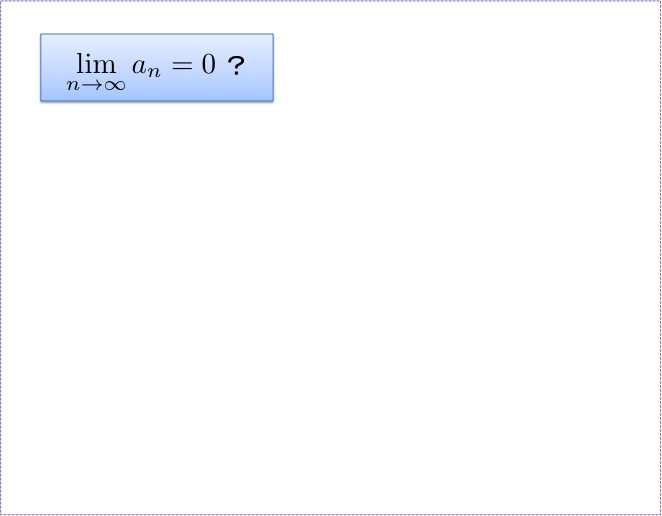
\includegraphics{./images/ch2/seriesCre/001.jpg}}}
% 		
% 		\only<3>{\resizebox{!}{6.8cm}{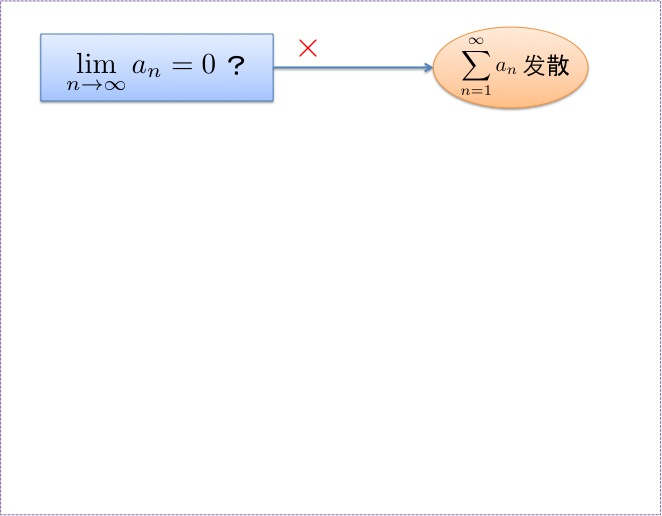
\includegraphics{./images/ch2/seriesCre/002.jpg}}}
% 		
% 		\only<4>{\resizebox{!}{6.8cm}{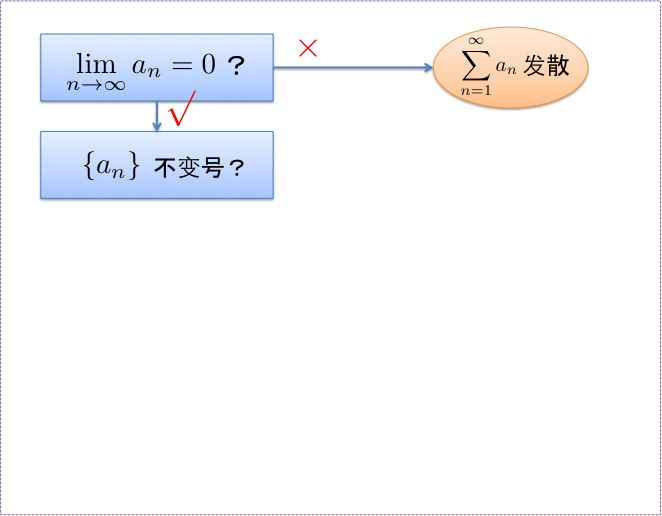
\includegraphics{./images/ch2/seriesCre/003.jpg}}}
% 		
% 		\only<5>{\resizebox{!}{6.8cm}{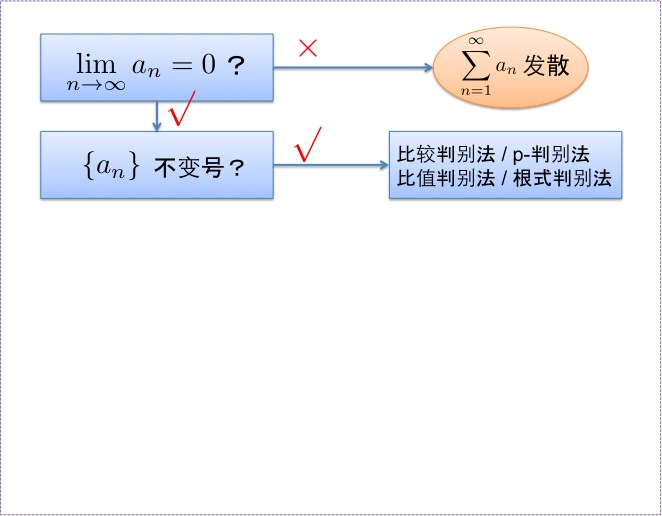
\includegraphics{./images/ch2/seriesCre/004.jpg}}}
% 		
% 		\only<6>{\resizebox{!}{6.8cm}{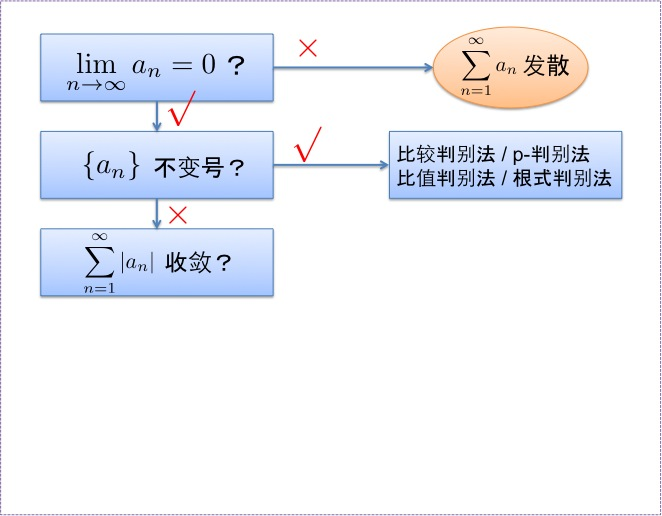
\includegraphics{./images/ch2/seriesCre/005.jpg}}}
% 		
% 		\only<7>{\resizebox{!}{6.8cm}{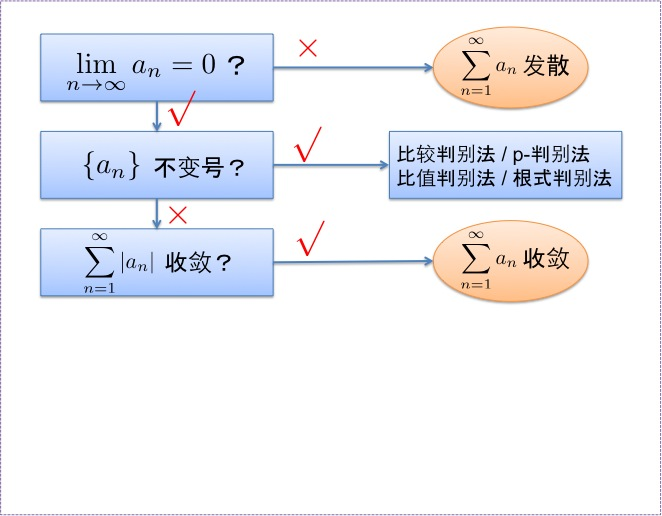
\includegraphics{./images/ch2/seriesCre/006.jpg}}}
% 		
% 		\only<8>{\resizebox{!}{6.8cm}{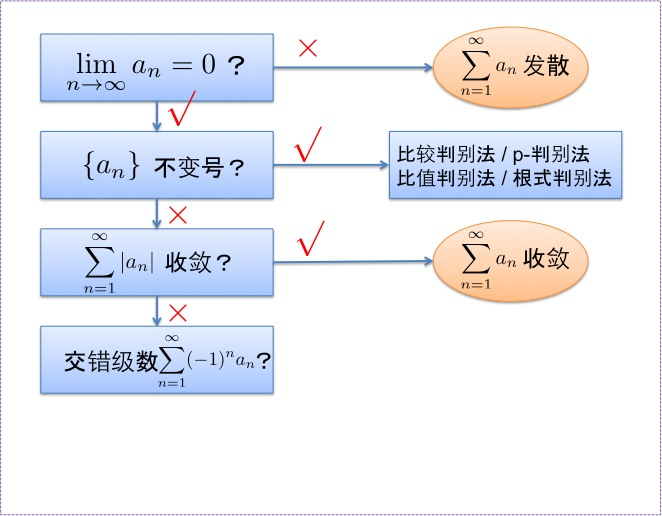
\includegraphics{./images/ch2/seriesCre/007.jpg}}}
% 		
% 		\only<9>{\resizebox{!}{6.8cm}{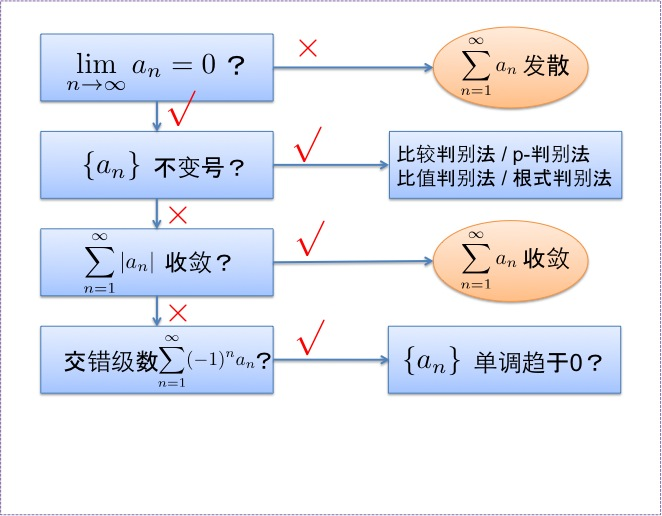
\includegraphics{./images/ch2/seriesCre/008.jpg}}}
% 		
% 		\only<10>{\resizebox{!}{6.8cm}{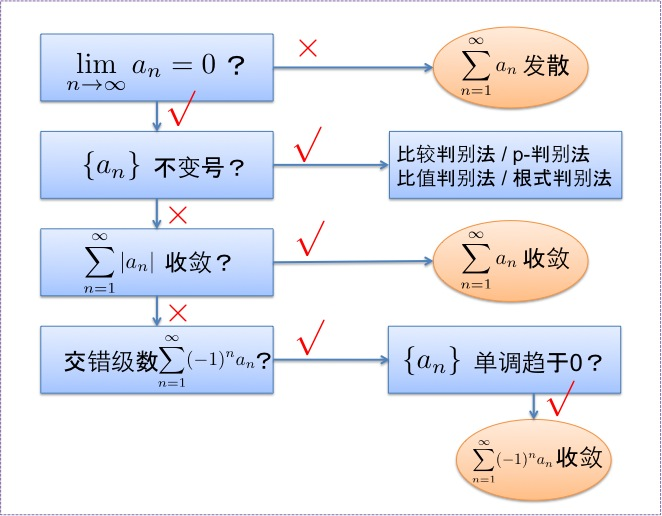
\includegraphics{./images/ch2/seriesCre/009.jpg}}}
% 		
% 		\only<11>{\resizebox{!}{6.8cm}{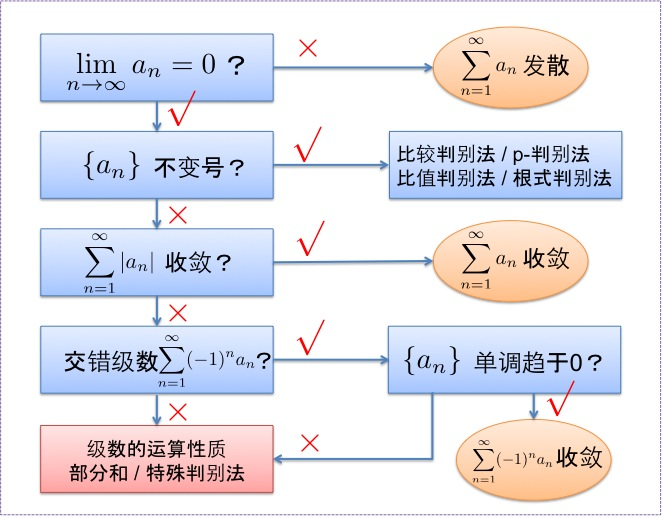
\includegraphics{./images/ch2/seriesCre/010.jpg}}}
% % 		\only<2>{\resizebox{!}{6.8cm}{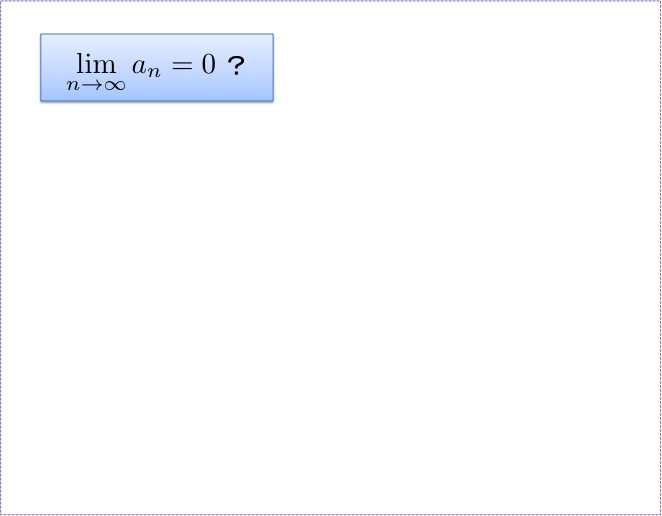
\includegraphics{./images/ch2/seriesCre/001.jpg}}}
% 	\end{center}
% \end{frame}

% \section{特殊判别法}

% \begin{frame}
% 	\linespread{1}
% 	\begin{block}{{\bf Gauss判别法}\hfill}
% 		设$a_n\geq 0\,(n=1,2,\ldots)$,且
% 		$$\df{a_{n+1}}{a_n}=1-\df pn+\df{\theta_n}{n^{1+\mu}},$$
% 		其中$\{\theta_n\}$有界,$\mu>0$。则
% 		当$p>1$时,$\sumn a_n$收敛;$p\leq 1$时,$\sumn a_n$发散。		
% 		\pause 
% 	\end{block}
% 	\begin{exampleblock}{{\bf 例11:}判断以下级数的敛散性\hfill}
% 		  $$\sumn\left[\df{(2n-1)!!}{(2n)!!}\right]^s\quad (s>0)$$ 
% 	\end{exampleblock}
% \end{frame}

% \begin{frame}[<+->]{小结}
% 	\linespread{1.5}
% 	\begin{enumerate}
% % 	  \item {\bf 概念:}$\sumn a_n=\limn\sum\limits_{i=1}^na_i$
% % 	  \item {\bf 性质:}
% % 	  \begin{itemize}
% % 	    \item $\sumn a_n$收敛$\Rightarrow\limn a_n=0$
% % 	    \item 改变有限项不改变级数的敛散性
% % 	    \item 无穷级数的求和次序不能随便更改
% % 	  \end{itemize}
% % 	  \item 级数收敛的“夹逼定理”
% 	  \item {\bf 正项级数:}
% 	  \begin{itemize}
% 	    \item $\sumn a_n$收敛$\Leftrightarrow\{S_n\}$有界
% 	    \item 比较判别法、比值判别法、根值判别法
% 	  \end{itemize}
% 	  \item {\bf 变号级数}
% 	  \item {\bf 特殊判别法*:}Raabe判别法、Dirichlet判别法、Abel判别法
% 	\end{enumerate}
% % 	\begin{exampleblock}{课后练习}
% % 	  \begin{itemize}
% % 	    \item 书面作业:{\b P76:3-6;\\
% % 	    \P86:1(2-4),3(3-8),5(2,4),6(1-3),8,9}
% % 	    \item 思考题:{\b P77-78:7,8;P87-88:10-15}
% % 	  \end{itemize}
% % 	\end{exampleblock}
% \end{frame}

% \section{极限与无穷级数习题课}

\begin{frame}{判断正误}
	\linespread{1.5}
% 	{\bf 判断以下说法的正误:}
	\begin{enumerate}\pause 
	  \item 若$a_n>0(n=1,2,\ldots)$,则\\
	  \centerline{$a_1-a_1+a_2-a_2+a_3-a_3+\ldots $}
	  收敛\pause \quad (\alert{$\times$})\pause
	  \item 若以上$\limn a_n=0$,则以上级数收敛\pause \quad
	  (\alert{$\surd$})\pause
	  \item $\sumn a_n$收敛,$\limn b_n=1\Rightarrow\sumn a_nb_n$收敛\pause
	  \quad (\alert{$\times$})\pause
	  \item $\sumn a_n$部分和有界,$\limn b_n=0\Rightarrow\sumn a_nb_n$收敛\pause
	  \quad (\alert{$\times$})
	\end{enumerate}
% 	\begin{exampleblock}{{\bf title}\hfill }
% 		\123
% 	\end{exampleblock}
\end{frame}

\begin{frame}{判断正误}
	\linespread{1.5}
% 	{\bf 判断以下说法的正误:}
	\begin{enumerate}\pause 
	  \addtocounter{enumi}{4}
	  \item 若$\limn\df{a_n}{b_n}=1$,则若$\sumn a_n$绝对收敛,$\sumn b_n$必收敛\pause \quad
	  (\alert{$\surd$})\pause
	  \item $\sumn a_n,\sumn b_n$绝对收敛$\Rightarrow\sumn (a_n+b_n)$绝对收敛\pause \quad
	  (\alert{$\surd$})\pause
	  \item $\sumn a_n,\sumn b_n$条件收敛$\Rightarrow\sumn (a_n+b_n)$条件收敛\pause \quad
	  (\alert{$\times$})\pause
	  \item 若$\sumn a_n^2$收敛,则$\sumn a_n^3$收敛\pause \quad
	  (\alert{$\surd$})
	\end{enumerate}
% 	\begin{exampleblock}{{\bf title}\hfill }
% 		\123
% 	\end{exampleblock}
\end{frame}

\begin{frame}[<+->]{判断下列级数的敛散性}
	\linespread{2.5}
	\begin{enumerate}
% 	  \item $\sumn\df{2^nn!}{n^n}$
	  \item $\df 1{a+b}+\df 1{2a+b}+\df 1{3a+b}+\ldots\quad (a>0,b>0)$
% 	  \item $\sumn\df{1!+2!+\ldots+n!}{n!}$
% 	  \item $\sumn\left[\df 1n-\ln\left(1+\df 1n\right)\right]$
% 	  \item $\sumn\df{\sqrt{n!}}{(2+\sqrt 1)(2+\sqrt 2)\ldots(2+\sqrt n)}$
	  \item $\sumn\left[\df 1n-\ln\left(1+\df 1n\right)\right]$
	  \item $\sumn\df{\sqrt{n+1}-\sqrt{n}}{n^p}\quad(p>0)$
% 	  \item $\sumn\df{n^{n+\frac 1{\,n\,}}}{\left(n+\df 1n\right)^n}$
	\end{enumerate}
\end{frame}

\begin{frame}[<+->]
	\linespread{2.5}
	\begin{enumerate}
	  \addtocounter{enumi}{4}
% 	  \item $\sumn\df{2^nn!}{n^n}$
% 	  \item $\sumn\left[\df 1n-\ln\left(1+\df 1n\right)\right]$
% 	  \item $\sumn\left[\df 1n-\ln\left(1+\df 1n\right)\right]$
% 	  \item $\sumn n!\left(\df{x}{n}\right)^n\quad (x>0)$
	  \item $\sumn n!\left(\df{x}{n}\right)^n\quad (x>0)$
	  \item $\sumn\df {a_n}{(1+a_1)(1+a_2)\ldots(1+a_n)}\quad(a_n\geq
	  0,n\in\mathbb{N})$
	  \item $\sumn\df{n^{n+\frac 1{\,n\,}}}{\left(n+\df 1n\right)^n}$
	\end{enumerate}
\end{frame}

% \begin{frame}{小结}
% 	\linespread{1.5}
% 	\begin{enumerate}
% 	  \item $\sumn a_n$收敛$\Rightarrow\limn a_n=0$
% % 	  \item 级数收敛的“夹逼定理”
% 	  \item {\bf 正项级数:}$a_n\geq 0\;(n\in\mathbb{N})$
% 	  \begin{itemize}
% 	    \item 正项级数$\sumn a_n$收敛$\Leftrightarrow\{S_n\}$有界
% 	    \item 比较判别法
% 	    \item 比值判别法
% 	    \item 根值判别法
% 	  \end{itemize}
% 	\end{enumerate}
% % 	\begin{exampleblock}{课后练习}
% % 	  \begin{itemize}
% % 	    \item 书面作业:{\b P76:3-6;\\
% % 	    \P86:1(2-4),3(3-8),5(2,4),6(1-3),8,9}
% % 	    \item 思考题:{\b P77-78:7,8;P87-88:10-15}
% % 	  \end{itemize}
% % 	\end{exampleblock}
% \end{frame}